%
% Aufbau und Validierung einer Konfigurationsdatei
% ===========================================================================
%

\chapter{Testdatenerstellung}
\label{chap:testdata}

Im Hinblick auf die Testdaten zum Testen der Compare-Funktionen sind zwei Kategorien von Testdaten zu unterscheiden: Testmodelle und Parameter der jeweiligen Compare-Funktion. Die in diesem Abschnitt beschriebene Erstellung von Testdaten bezieht sich dabei auf die Erstellung von Testmodellen.

\section{Testmetamodell}
Für die Erstellung von Testmodellen wurde ein eigenes Metamodell, im Folgenden als Testmetamodell bezeichnet, entworfen (Bundle  \texttt{org.sidiff.common.testmetamodel}). Das Testmetamodell ist dabei möglichst schlank gehalten, beinhaltet aber dennoch die für reale Metamodelle typischen Strukturen: Komponenten (Blöcke) und gerichtete Beziehungen (Linien) zwischen den Komponenten. Zudem wurde darauf geachtet, alle primitiven EMF-Datentypen zu verwenden. Abbildung \ref{img_testmetamodel} zeigt das Testmetamodell in der bekannten Ecore-Diagramm-Notation.

\begin{figure}
	\centering	
	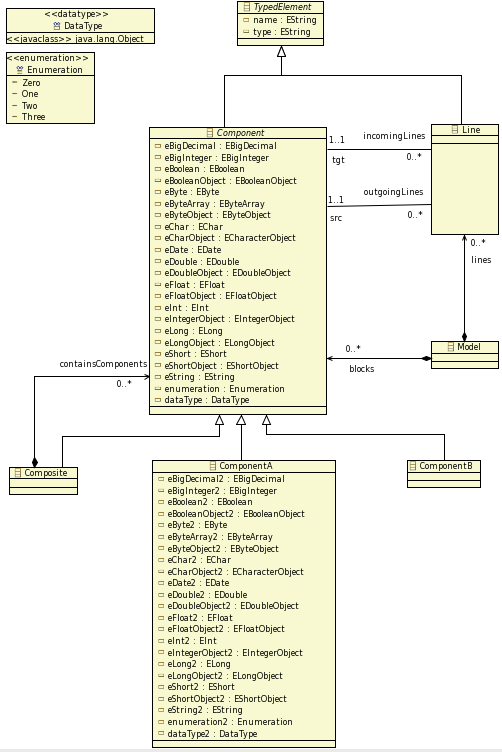
\includegraphics[scale=0.8]{img/testmetamodel.png}
	% testmetamodel.png: 502x752 pixel, 96dpi, 13.28x19.89 cm, bb=0 0 376 564
	\label{img_testmetamodel}
	\caption{Testmetamodell}
\end{figure}

\section{Erstellung von Testmetamodell-Instanzen}
Für die Erstellung von Testmetamodell-Instanzen exisitieren verschiedene Möglichkeiten, von denen hier zwei näher betrachtet werden sollen:
\begin{enumerate}
 \item Mittels des durch EMF bereit gestellten, generischen Ecore-Editors. Hat den Nachteil, dass es teilweise mühsam sein kann, die Graph-Struktur der Modelle zu erfassen. Das gilt sowohl für die Erstellung der Testdaten, als auch für die Nachvollziehbarkeit der einzelnen Testfälle.
 \item Instanzen werden in UML-Notation mittels eines UML-Tools spezifiziert und über einen Konverter nach EMF transformiert.
\end{enumerate}
Aus Gründen der Nachvollziehbarkeit und der leichteren Erstellung von Testmodellen werden wir die 2.te Variante anwenden. Als UML-Werkzeug ist der IBM Rational Software Modeler (RSM) in der Version 7.5 zu benutzen. Im Folgenden werden die einzelnen Schritte zur Erstellung von Testmodellen beschrieben.


\subsection{Modellerstellung in RSM}
Alle Testmodelle sind im RSM zu erstellen. Hierzu existieren zwei RSM-Projekte, TestmetamodelProfile und TestModels, welche im Verzeichnis \texttt{rsm/workspace} des Bundles \texttt{org.sidiff.common.testmodels} zu finden sind. Das Projekt TestmetamodelProfile definiert einige zur Identifikation von Komponenten benötigte Stereotypen (s. unten). Die eigentlichen Testmodelle werden im Projekt TestModels spezifiziert. 

\subsubsection{Pakethierarchie} 
Testmodelle werden in einer Pakethierarchie organisiert, welche folgenden Konventionen genügt (s. Abbildung \ref{img:package-hierarchie}):

\begin{itemize}
 \item Auf oberster Ebene befindet sich das Paket, welches die JUnit-Testfälle beinhaltet. Das Paket heißt wie das jeweilige OSGI-Bundle (z.B. org.sidiff.compare.comparefunctions.emf.test)
 \item Auf der nächsttieferen Ebene befindet sich das Paket, welche alle Testdaten für eine spezielle Compare-Funktion Test-Suite (z.B. CompareAttributeUsingLCSTest) beinhaltet.
 \item Auf der nächsten Hierarchie-Ebene befinden sich Pakete für alle Testfälle. Diese Pakete werden entsprechend dem Namensmuster $testcase_<NR.>$ benannt, wobei $<NR.>$ einer sequenziell hochgezählten Nummer entspricht.
 \item Für jeden Testfall werden schließlich die Eingabemodelle (in der Regel zwei) spezifiziert, welche sich in Unterpakten model-1 bzw. model-2 befinden. 
\end{itemize}

\begin{figure}
	\centering
 	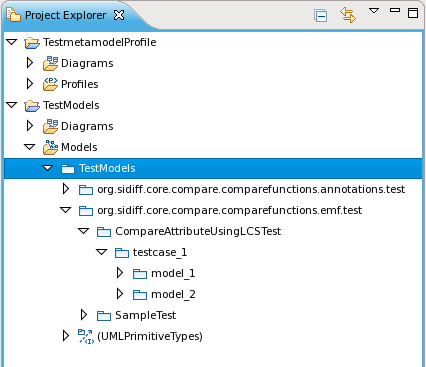
\includegraphics[scale=0.8]{img/package-hierarchie.png}
	\label{img:package-hierarchie}
	\caption{Exemplarische Paket-Hierarchie}
\end{figure}

\subsubsection{Spezifikation der eigentlichen Testmodelle}
Die eigentlichen Testmodelle werden in den oben beschriebenen Paketen model-1 bzw. model-2 spezifiziert. Zur grafischen Visualisierung ist ein Klassendiagramm zu verwenden. Abbildung \ref{img:sample-instance} zeigt ein Exemplarisches Testmodell in Klassendiagramm-Notation, Abbildung \ref{img:sample-instance-structure} die dazugehörige Modellstruktur, wie sie im RSM im Projekt-Explorer dargestellt wird. 

\begin{figure}
	\centering
 	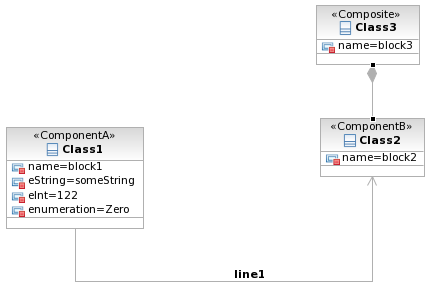
\includegraphics[scale=0.8]{img/sample-instance.png}
	\label{img:sample-instance}
	\caption{Exemplarisches Testmodell in UML-Klassendiagramm Notation}
\end{figure}

\begin{figure}
	\centering
 	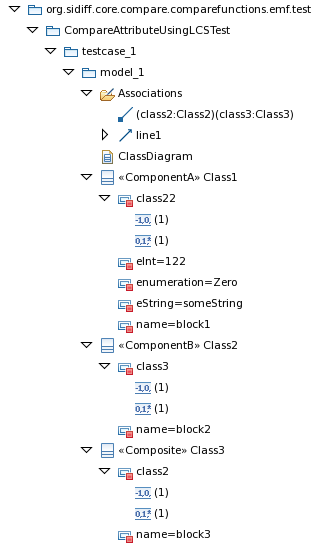
\includegraphics[scale=0.8]{img/sample-instance-structure.png}
	\label{img:sample-instance-structure}
	\caption{Exemplarische Modellstruktur}
\end{figure}

Die im Testmetamodell definierten Metaklassen werden durch folgende UML-Konstrukte umgesetzt:
\begin{itemize}
 \item ComponentA: Entspricht einer Klasse mit dem Stereotyp ComponentA (welcher in TestmetamodelProfile als Erweiterung der UML-Metaklasse Class definiert ist).
 \item ComponentB: Entspricht einer Klasse mit dem Stereotyp ComponentB (welcher in TestmetamodelProfile als Erweiterung der UML-Metaklasse Class definiert ist).
 \item Composite: Entspricht einer Klasse mit dem Stereotyp Composite (welcher in TestmetamodelProfile als Erweiterung der UML-Metaklasse Class definiert ist). Die Beziehung containsComponent ist durch eine Kompositionsbeziehung umzusetzen.
 \item Line: Lines werden durch gerichtete Assoziationen abgebildet. Rollennamen und Kardinalitäten brauchen nicht spezifiziert zu werden.
\end{itemize}

\subsubsection{Einschränkungen und Konventionen}
Folgende Einschränkungen und Konventionen sind zu beachten:
\begin{itemize}
 \item Attribute: Die Zuordnung von durch das Testmetamodell definierten Attributen und Attributwerten geschieht über die Benennung eines UML-Attributs nach folgendem Muster: $<attr-name>=<attr-value>$, wobei $<attr-name>$ dem Namen eines Attributs im Testmetamodell und $<attr-value>$ dem dazugehörigen Attributwert entspricht. Für einen Testfall nicht relevante Attribute müssen nicht spezifiziert zu werden. 
 \item Eindeutige Identifizierer: Modellelemente müssen eindeutig identifizierbar sein. Für alle Komponenten (ComponentA, ComponentB, Composite) ist daher das Attribut name unbedingt anzugeben. Auch Lines müssen identifizierbar sein. Als eindeutiger Identifizierer dient hier der Assoziationsname.
\end{itemize}

\subsection{Modellexport und Generierung von EMF-Modellen}
Um aus den im RSM erstellten UML-Modellen EMF-Modelle als die eigentlichen Testdaten der JUnit-Testfälle zu erhalten, sind diese zunächst im Eclipse UML2-Format zu exportieren und anschließend durch einen Konverter nach EMF zu transformieren. Beide Schritte werden im Folgenden beschrieben.

\subsubsection{Modellexport} Der Modellexport untergliedert sich in die folgenden Schritte:\\

\textbf{Schritt 1:} Rechtsklick auf das RSM-Projekt TestModels $>$ Export.\\

\textbf{Schritt 2:} Auswahl der Kategorie Other $>$ UML 2.1 Model (s. Abb. \ref{img:export-wizard-1}).\\
\begin{figure}
	\centering
 	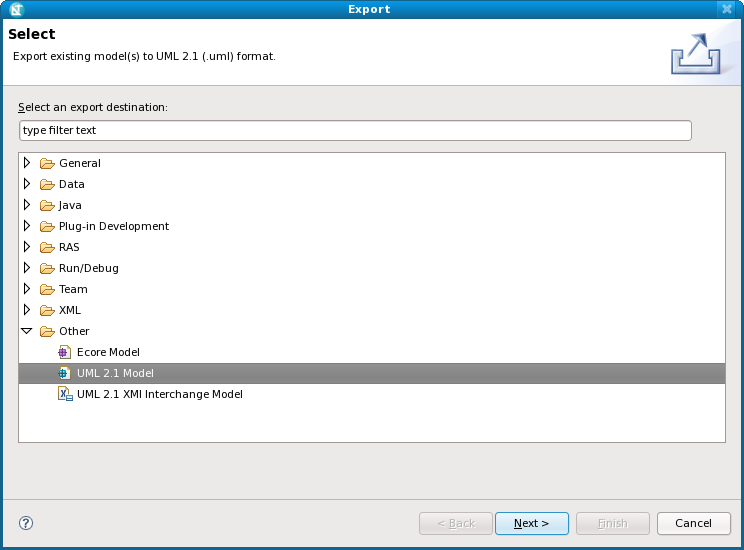
\includegraphics[scale=0.6]{img/export-wizard-1.png}
	\label{img:export-wizard-1}
	\caption{Export Wizard (1)}
\end{figure}

\textbf{Schritt 3:} Auswahl des zu exportierenden Modells und des Zielverzeichnisses, für welches das Verzeichnis \texttt{rsm/export} im Bundle \texttt{org.sidiff.common.testmodels} zu wählen ist. \textbf{Wichtig:} Unbedingt die Option Export applied profiles aktivieren! (s. Abb. \ref{img:export-wizard-2}).\\
\begin{figure}
	\centering
 	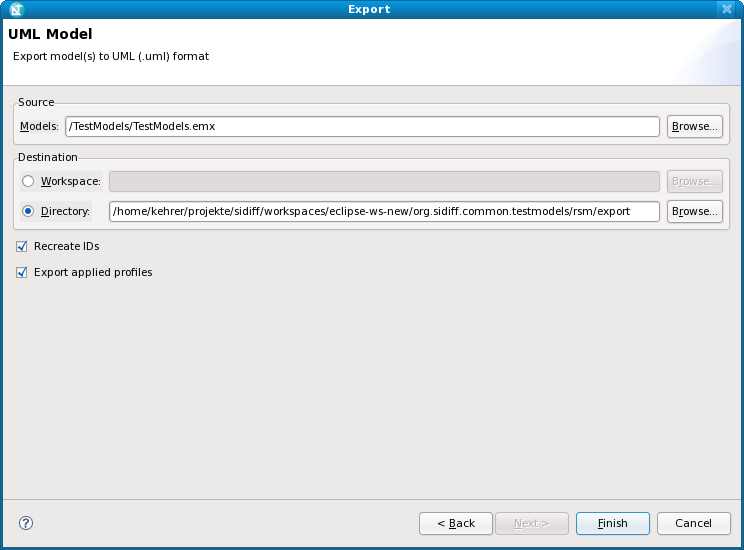
\includegraphics[scale=0.6]{img/export-wizard-2.png}
	\label{img:export-wizard-2}
	\caption{Export Wizard (2)}
\end{figure}


\subsubsection{Generierung von EMF-Modellen}
Um EMF-Modelle zu generieren, muss eine OSGI-Konsole mit dem Bundle org.sidiff.common.testmodels gestartet werden. Dieses nimmt ein Kommando generate $<WORKSPACE-URI>$ entgegen, wobei $<WORKSPACE-URI>$ den Betriebssystem-absoluten Pfad zu dem für die SiDiff-Entwicklung genutzten Eclipse-Workspace darstellt. Um die ständige Eingabe dieses Parameters zu vermeiden, kann in der Klasse \texttt{TestdataGeneratorCommandProvider} im Bundle und gleichnamigen Paket \texttt{org.sidiff.common.testmodels} ein neues Kommando spezifiziert werden, welches die private Methode generate(String workspaceUri) aufruft. Beispiel: 
\begin{lstlisting}
public void _generateTK(CommandInterpreter commandInterpreter) throws Exception {
	generate("/home/kehrer/projekte/sidiff/workspaces/eclipse-ws-new");
}
\end{lstlisting}

Die generierten EMF-Modelle werden in den jeweiligen Bundles zum Testen der Compare-Funktionen abgelegt.